\documentclass[conference]{IEEEtran}
\IEEEoverridecommandlockouts

\usepackage[T1]{fontenc}
\usepackage[utf8]{inputenc}
\usepackage[shorthands=off,turkish]{babel}
\usepackage{amsmath,amssymb}
\usepackage{graphicx}
\usepackage{booktabs}
\usepackage{array}
\usepackage{float}
\usepackage{url}
\usepackage[hidelinks]{hyperref}

\graphicspath{{figures/}}
\newcommand{\isp}{I_{\mathrm{sp}}}

\begin{document}

\title{Kalabalıkta İnsan-Merkezli Navigasyon için V38:\\
SNCP--PPO Üzerinde Eğitimsiz Eylem Kalkanı}

\author{\IEEEauthorblockN{Orkun Koray Güngör}
\IEEEauthorblockA{\textit{Mekatronik Mühendisliği Bölümü}\\
\textit{Bursa Teknik Üniversitesi}\\
Bursa, Türkiye\\
orkun9312@gmail.com}
\thanks{Kaynak kodu, Colab notebook'u ve deney artefaktları:
\url{https://github.com/heimdilon/sncp-ppo-crowdnav}}}

\maketitle

\begin{abstract}
Kalabalıkta sosyal navigasyon, öğrenilmiş rota seçimi ile yürütme zamanı güvenliğini aynı anda gerektirir.
Bu çalışma, SNCP--PPO tabanlı kalabalık navigasyon projesinin nihai V38 sistemini raporlar. Önceki sürümler,
ön-MLP gömmesi, yoğunluk müfredatı, mean+max havuzlama ve Beta eylem dağılımı ile güçlü bir v34 tabanı üretmiş;
ancak yüksek yoğunlukta kalan hata kipinin büyük ölçüde çarpışma olduğunu göstermiştir. V38 bu nedenle yeni
bir PPO eğitimi yapmaz. Kilitli v34 Beta checkpoint'inin deterministik eylemi alınır; kısa-horizon sabit-hız
öngörüsüyle çarpışma riski kontrol edilir; yalnızca riskli durumda daha düşük riskli bir alternatif eylem
yürütülür.
Bu eğitimsiz action-shield katmanı, aynı checkpoint, aynı değerlendirme tohumları ve aynı bölümler üzerinde
ham v34 ile karşılaştırıldığında N=20 başarıyı \%86.0'dan \%98.8'e çıkarır ve çarpışmayı \%13.2'den \%0.4'e
indirir. Dürüst 5-değerlendirme-tohumu havuzunda (250 bölüm/yoğunluk) final V38 başarıları N=5/10/15/20 için
\%99.6/\%99.6/\%99.6/\%98.8, çarpışmalar ise \%0.0/\%0.0/\%0.4/\%0.4'tür. Böylece V38, yeni checkpoint
eğitmeden, öğrenilmiş sosyal rotayı koruyup çarpışma sınırındaki eylemi düzelten pratik bir final sistem adayı
sunar.
\end{abstract}

\begin{IEEEkeywords}
sosyal navigasyon, kalabalıkta robot hareketi, PPO, SNCP, action shield, çarpışma-risk filtresi
\end{IEEEkeywords}

% =====================================================================
\section{Giriş}
% =====================================================================
Kalabalıkta mobil robot navigasyonu, yalnızca geometrik olarak kısa bir yol bulmak değildir. Robot hedefe
ulaşırken yayaların hareketini hesaba katmalı, çarpışmadan kaçınmalı ve yoğunluk arttıkça güvenli geçiş
fırsatlarını değerlendirmelidir. Referans aldığımız SNCP--PPO yaklaşımı, bu problemi robot ve yayalar
arasındaki etkileşimi uzay-zamansal bir grafa dönüştürerek çözer; Liquid Time-Constant ve Neural Circuit
Policy kodlayıcılarıyla etkileşimleri işler ve son eylemi PPO ile öğrenir~\cite{ao2026sncp,hasani2021ltc,lechner2020ncp,schulman2017ppo}.
Yaya hareketi için CrowdNav çizgisindeki görünmez-robot varsayımı ve ORCA kalabalık dinamiği kullanılır
~\cite{chen2019crowdnav,vandenberg2011orca}.

Projedeki erken amaç, referans makaledeki yüksek başarı oranına saf öğrenilmiş politika ile yaklaşmaktı.
Bu süreçte birçok mimari ve eğitim kararı test edildi. Sonuçta v34 Beta politikası güçlü ve dengeli bir taban
oldu: sınırlı eylem uzayında Beta dağılımı, kırpılmış Gauss politikasına göre daha uygun bir yürütme davranışı
sağladı~\cite{chou2017beta}. Buna rağmen yüksek yoğunlukta kalan başarısızlıkların çoğu zaman aşımı değil,
çarpışmaydı. Bu gözlem, yeni bir büyük eğitim koşusu yerine yürütme zamanı çarpışma-risk filtresini daha
savunulabilir son adım yaptı.

Bu makalenin odağı bu son adımdır. V38, v34 checkpoint'ini değiştirmez; öğrenilmiş rotayı korur ve sadece
kısa-horizon çarpışma riski olan eylemleri değiştirir. Katkılarımız:
\begin{itemize}
\item Kilitli v34 Beta politikasının üzerine eğitimsiz, kısa-horizon action-shield katmanı ekliyoruz.
\item Kalkan etkisini aynı checkpoint, aynı değerlendirme tohumları ve aynı bölüm bankası üzerinde ham v34'e
karşı izole ediyoruz.
\item Dürüst 5-değerlendirme-tohumu havuzunda final V38 sisteminin N=20 challenging başarısını \%98.8'e
çıkardığını ve
çarpışmayı \%0.4'e indirdiğini gösteriyoruz.
\item Raporu eski ablation figürlerine dayandırmadan, V38 final sistemine özel yeni tablolar ve görsellerle
sunuyoruz.
\end{itemize}

Bu yaklaşım, öğrenen ajanın eylemini izleyip yalnızca güvenlik ihlali öngörüldüğünde düzelten
``shielded reinforcement learning'' fikrine yakındır~\cite{alshiekh2018shielding}. Bununla birlikte V38,
zamansal mantıkla sentezlenmiş biçimsel bir kalkan veya ileri-değişmezlik garantisi veren bir
control-barrier-function denetleyicisi değildir~\cite{ames2017cbf}. Buradaki amaç, kilitli v34 politikasının
iyi sosyal rota kararını korurken, kısa ufukta açıkça riskli görünen sürekli eylemi pratik bir aday eylem
aramasıyla değiştirmektir.

% =====================================================================
\section{Yöntem}
% =====================================================================
\begin{figure}[H]
\centering
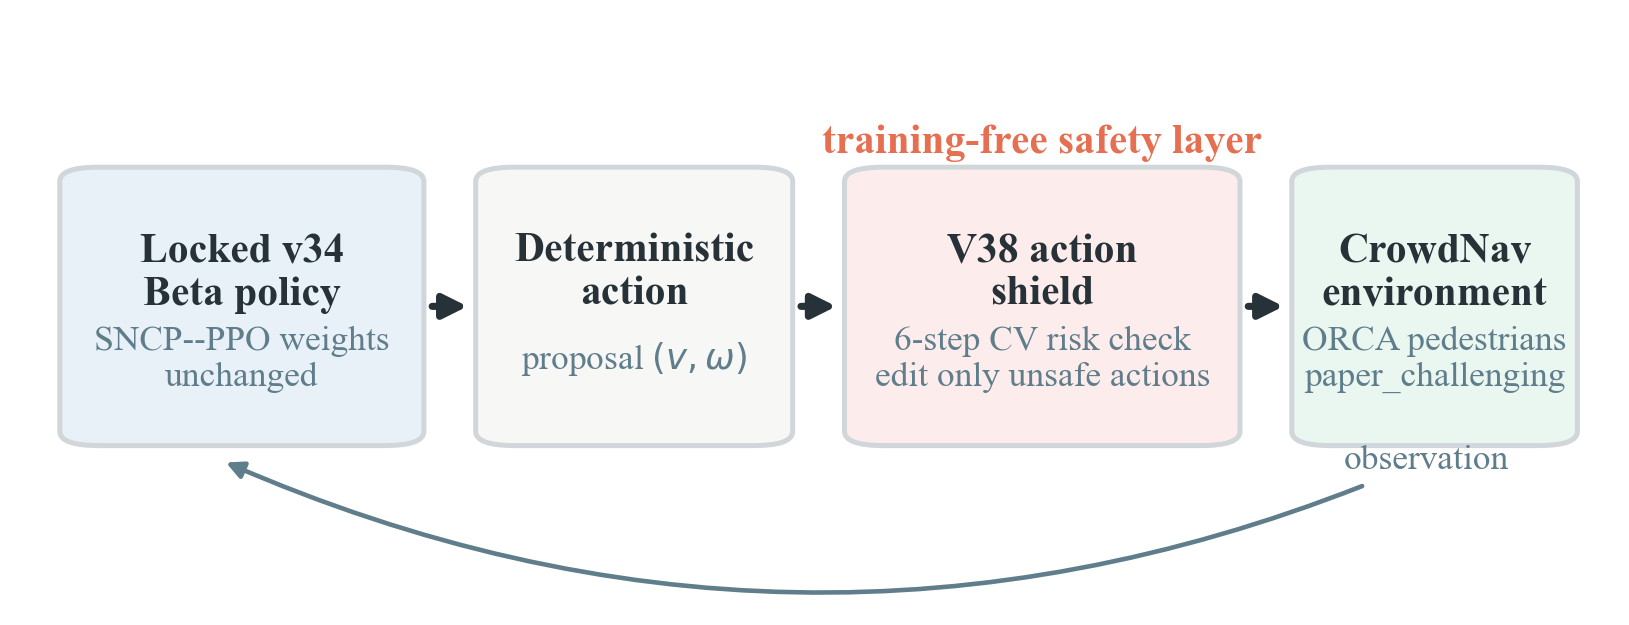
\includegraphics[width=\columnwidth]{fig_v38_pipeline.png}
\caption{V38 yürütme hattı. Kilitli v34 Beta politikası sosyal rota üretir; V38 kalkanı yalnızca kısa-horizon
çarpışma riski görüldüğünde eylemi değiştirir. Checkpoint ağırlıkları değişmez.}
\label{fig:pipeline}
\end{figure}

\subsection{Kilitli v34 Beta politikası}
Taban politika, SNCP--PPO mimarisinin v34 Beta checkpoint'idir. Bu checkpoint, robotun kalabalıkta doğrudan
beeline yerine kavisli ve sosyal açıdan makul rotalar üretmesini sağlar. V34'ün bu çalışmadaki rolü sabittir:
ağırlıkları değiştirilmez, yeniden eğitim yapılmaz ve V38'in öğrenilmiş bileşeni olarak korunur. Böylece
V38'in etkisi, politika mimarisindeki yeni bir öğrenmeden değil, yalnız yürütme zamanı çarpışma-risk
filtresinden gelir.

\subsection{V38 action shield}
V38, deterministik politika eylemini bir çarpışma-risk filtresinden geçirir. İş akışı Şekil~\ref{fig:pipeline}'da
özetlenmiştir. Politika önce $(v,\omega)$ eylemini önerir. Kalkan, robot ve yayalar için 6 adımlık sabit-hız
öngörüsü yapar. Öngörü ufku içinde robot--yaya mesafesi çarpışma sınırını ihlal etmiyorsa eylem aynen
yürütülür. Risk varsa, sınırlı bir aday eylem kümesi taranır ve çarpışma riskini azaltırken hedefe ilerlemeyi
mümkün olduğunca koruyan alternatif seçilir.

Kalkanın kritik özelliği seçici olmasıdır: her adımda politika çıktısını yeniden planlamaz, yalnızca kısa
ufukta risk görüldüğünde devreye girer. Bir politika eylemi $a_\pi=(v_\pi,\omega_\pi)$ için önce robotun
mevcut pozu, yayaların mevcut konumları ve yayaların anlık hızları alınır. Robotun $a_\pi$ ile, yayaların ise
sabit hızla ilerlediği varsayılarak $H=6$ adımlık bir mikro-rollout yapılır. Bu rollout'taki en küçük
robot--yaya mesafesi $d_{\min}$ ise kalkan açıklığı
\begin{equation}
\rho(a_\pi)=d_{\min}-d_{\mathrm{coll}}
\end{equation}
olarak hesaplanır. Burada $d_{\mathrm{coll}}$ ortamın robot--yaya çarpışma eşiğidir. Eğer
$\rho(a_\pi)\geq m$ ise, yani öngörülen açıklık risk marjı $m$'den büyükse, $a_\pi$ değiştirilmez.

Riskli durumda kalkan küçük bir eylem kafesi dener. Doğrusal hız kafesi durma, çeyrek/yarım/üç-çeyrek/tam
hız ve politika hızının yarım/üç-çeyrek/tam değerlerini içerir. Açısal hız kafesi ise maksimum sağ/sol dönüş,
yarım maksimum sağ/sol dönüş, düz gitme ve politikanın önerdiği dönüşten oluşur. Her aday aynı mikro-rollout
ile değerlendirilir ve aşağıdaki maliyetin en küçüğünü veren eylem seçilir:
\begin{equation}
\begin{split}
J(a) ={}& \lambda_c \mathbf{1}[\rho(a)<0]
+ \lambda_s \max(0,m-\rho(a))^2
- \lambda_p \Delta d_g(a) \\
&+ \lambda_d \|a-a_\pi\|_{\mathrm{norm}}
+ \lambda_v \left(1-\frac{v}{v_{\max}}\right).
\end{split}
\end{equation}
Bu maliyet çarpışmayı baskın şekilde cezalandırır, öngörülen açıklık azaldığında ek ceza verir, hedefe
ilerlemeyi ödüllendirir ve v34 politikasının önerdiği eylemden gereksiz sapmayı sınırlar. Bu nedenle V38,
tam bir yörünge planlayıcı veya yeni bir öğrenilmiş politika değildir; v34'ün sosyal rota kararını koruyan,
yalnızca çarpışma sınırındaki eylemleri düzelten yürütme zamanı risk filtresidir.

Bu çalışmada kullanılan sayısal değerler $H=6$, $m=0.0$, $\lambda_c=1000.0$, $\lambda_s=20.0$,
$\lambda_p=1.0$, $\lambda_d=0.05$ ve $\lambda_v=0.02$'dir. Katsayılar ayrı bir öğrenme veya geniş ızgara
aramasıyla ayarlanmamıştır; çarpışmayı baskın öncelik yapan, sonra açıklık, hedef ilerlemesi,
politika eyleminden sapma ve gereksiz yavaşlama arasında sezgisel bir sıralama kuran sabit mühendislik
parametreleri olarak seçilmiştir.

Bu tasarım bilinçli olarak küçüktür. Eğitim gerektirmez, v34'ün başarılı sosyal rota davranışını bozmaz ve
yalnızca teşhis edilen hata kipine, yani çarpışma sınırındaki yanlış eylemlere müdahale eder.

% =====================================================================
\section{Deney Protokolü}
% =====================================================================
Ana değerlendirme \texttt{paper\_challenging} senaryosunda yapılır: $15\times15$~m arena, ORCA yayalar,
görünmez robot ve 1.0~m/s robot/yaya hız rejimi. Yoğunluklar $N=\{5,10,15,20\}$ olarak seçilir.

\begin{table}[H]
\centering
\caption{V38 final deney kurulumu.}
\label{tab:setup}
\small
\begin{tabular}{@{}>{\raggedright\arraybackslash}p{0.30\columnwidth}>{\raggedright\arraybackslash}p{0.64\columnwidth}@{}}
\toprule
\textbf{Bileşen} & \textbf{Ayar} \\
\midrule
Senaryo & \texttt{paper\_challenging} \\
Yoğunluklar & 5, 10, 15, 20 yaya \\
Değerlendirme & 5 eval tohumu $\times$ 50 bölüm = 250 bölüm/yoğunluk \\
Taban politika & v34 Beta checkpoint \\
Karşılaştırma & Ham v34 vs v38 shield \\
Robot/yaya hızı & 1.0~m/s \\
Kalkan ufku & 6 adım sabit-hız öngörüsü \\
Kalkan marjı & 0.0 \\
İstatistik & Wilson GA; havuzlanmış $z$ + Bonferroni $\alpha=0.0125$ \\
\bottomrule
\end{tabular}
\end{table}

Kalkan etkisini izole etmek için ham v34 ve V38 aynı checkpoint, aynı değerlendirme tohumları ve aynı bölüm
bankası üzerinde
karşılaştırılır. Bu düzende tek fark, yürütme zamanı action shield katmanıdır. Başarı, çarpışma ve zaman aşımı
bölüm yüzdesi olarak raporlanır; başarılı bölümlerin ortalama adım sayısı, sosyal rotanın korunup korunmadığını
yorumlamak için ayrıca verilir. Buradaki beş tohum, yeni PPO eğitim tohumları değil, kilitli tek v34 checkpoint
üzerinde kullanılan değerlendirme tohumlarıdır. Ana tablolardaki 250 bölüm/yoğunluk sonuçları
\texttt{paper\_data/v34\_multiseed\_result.json} ve \texttt{paper\_data/v38\_multiseed\_result.json}
dosyalarından gelir; \texttt{eval\_v38} artefaktları ise ek rapor ve yörünge görselleri için korunur.

Kalkan maliyeti ayrıca yerel CPU üzerinde, yalnız \texttt{shield\_action} çekirdeğini kapsayan 1000 çağrılık bir
ön mikro-ölçümle kontrol edildi. Aynı $H=6$ ayarıyla medyan süre N=5/10/15/20 için yaklaşık
0.108/0.108/0.113/0.123~ms, 95. yüzdelik süre ise 5.6/5.8/5.9/6.6~ms ölçüldü. Bu ön ölçüm, kalkan çekirdeğinin
10~Hz kontrol döngüsündeki 100~ms karar bütçesinin altında kalabileceğini gösterir; ancak politika çıkarımı,
algılama, ROS iletişimi ve gerçek robot entegrasyonu bu süreye dahil değildir.

RL sonuçlarının tohum ve bölüm seçimine duyarlı olabildiği bilindiğinden~\cite{henderson2018matters,agarwal2021precipice},
p-değerleri Wilson güven aralıklarıyla birlikte ve destekleyici karar ölçütü olarak yorumlanır. Aynı bölüm
bankası kullanıldığı için ideal ek analiz, bölüm-düzeyi eşleşmiş sonuçlardan McNemar testi veya paired bootstrap
güven aralığı üretmektir; mevcut artefaktlarda karar, havuzlanmış iki-oranlı $z$ testi ve Bonferroni düzeltmesi
ile raporlanmıştır.

% =====================================================================
\section{Sonuçlar}
% =====================================================================
\subsection{Kalkan etkisi: ham v34'ten V38'e}
Tablo~\ref{tab:shield_success}, Tablo~\ref{tab:shield_collision} ve Şekil~\ref{fig:effect}, V38 kalkanının
doğrudan etkisini gösterir. Havuzlanmış iki-oranlı $z$ testine göre kalkan N=10, N=15 ve N=20'de başarıyı
Bonferroni eşiğinde artırır; çarpışmayı dört yoğunlukta da aynı eşikte azaltır.
N=20'de başarı \%86.0'dan \%98.8'e çıkar, çarpışma \%13.2'den \%0.4'e iner. Zaman aşımı \%0.8 ve altında
kaldığı için iyileşme robotu durdurarak değil, çarpışma sınırındaki eylemleri düzelterek gelir.

\begin{table}[H]
\centering
\caption{V38 action shield başarı etkisi. Değerler yüzde; kalın p-değerleri havuzlanmış $z$ testinde
Bonferroni eşiğini geçer ($p<0.0125$).}
\label{tab:shield_success}
\small
\begin{tabular}{@{}lrrrr@{}}
\toprule
\textbf{N} & \textbf{v34} & \textbf{V38} & \textbf{$\Delta$} & \textbf{p} \\
\midrule
5  & 96.8 & 99.6 & +2.8  & 0.019 \\
10 & 92.8 & 99.6 & +6.8  & \textbf{$<10^{-3}$} \\
15 & 91.2 & 99.6 & +8.4  & \textbf{$<10^{-3}$} \\
20 & 86.0 & 98.8 & +12.8 & \textbf{$<10^{-3}$} \\
\bottomrule
\end{tabular}
\end{table}

\begin{table}[H]
\centering
\caption{V38 action shield çarpışma ve zaman aşımı etkisi. Çarpışma için negatif $\Delta$ daha iyidir; kalın
p-değerleri havuzlanmış $z$ testinde Bonferroni eşiğini geçer ($p<0.0125$).}
\label{tab:shield_collision}
\small
\begin{tabular}{@{}lrrrrr@{}}
\toprule
\textbf{N} & \textbf{v34 ç.} & \textbf{V38 ç.} & \textbf{$\Delta$ ç.} & \textbf{p} & \textbf{V38 z.aş.} \\
\midrule
5  & 2.8  & 0.0 & -2.8  & \textbf{0.008}       & 0.4 \\
10 & 7.2  & 0.0 & -7.2  & \textbf{$<10^{-3}$} & 0.4 \\
15 & 8.8  & 0.4 & -8.4  & \textbf{$<10^{-3}$} & 0.0 \\
20 & 13.2 & 0.4 & -12.8 & \textbf{$<10^{-3}$} & 0.8 \\
\bottomrule
\end{tabular}
\end{table}

\begin{figure}[H]
\centering
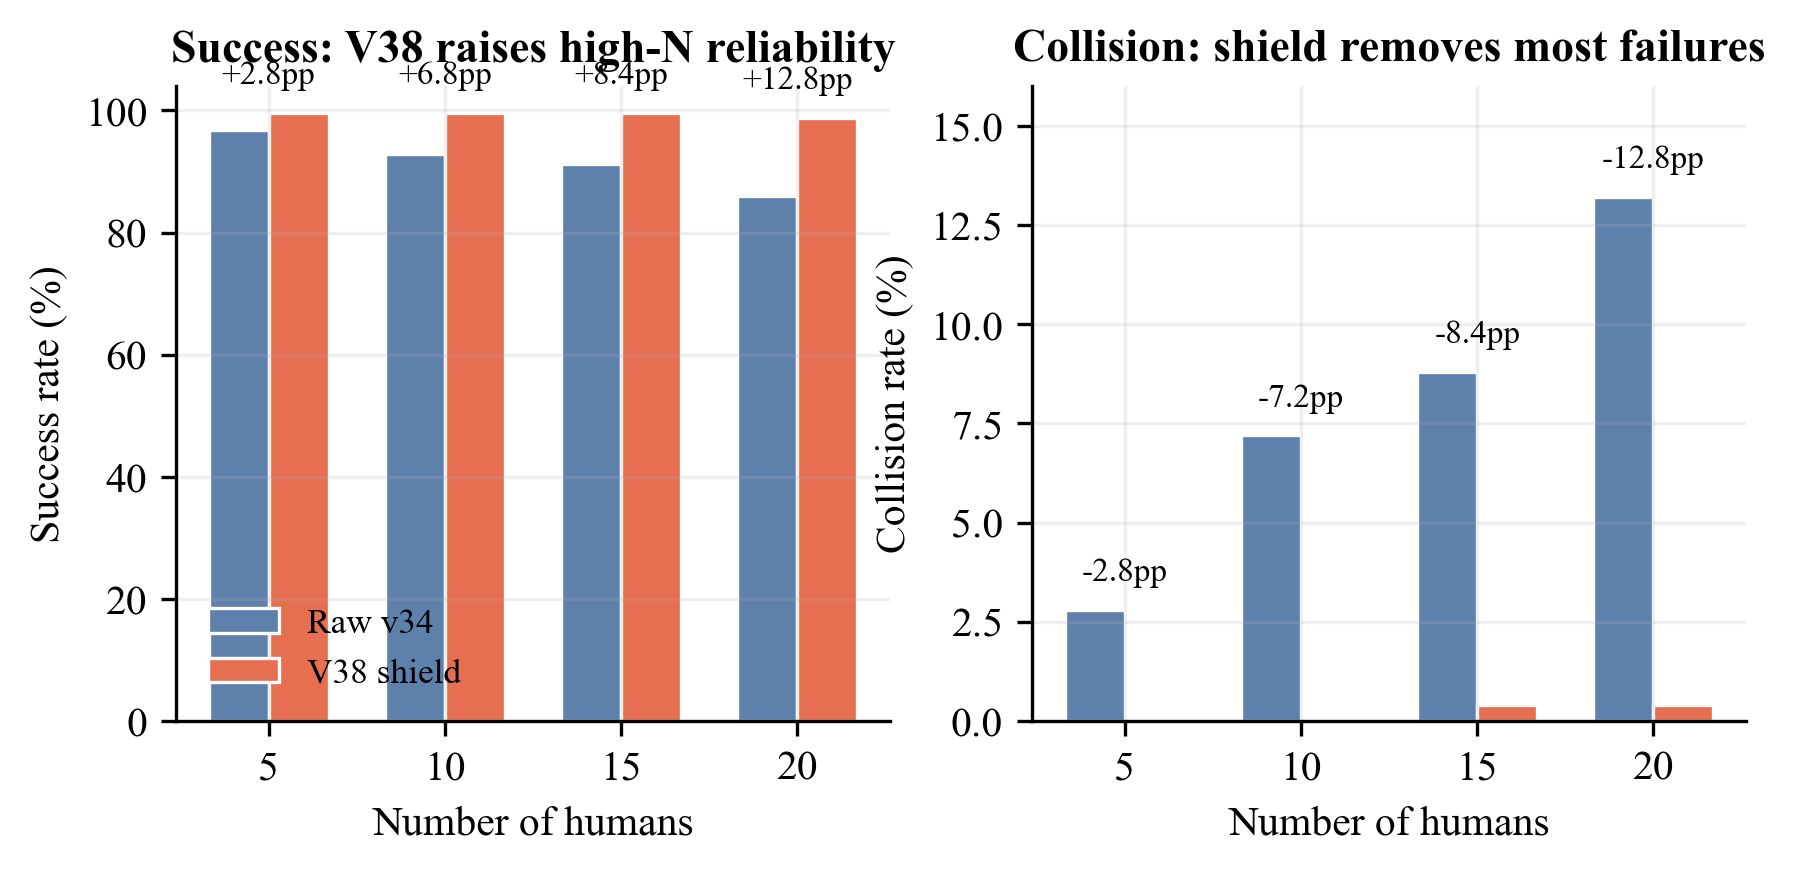
\includegraphics[width=\columnwidth]{fig_v38_shield_effect.png}
\caption{V38 kalkanının izole etkisi. Sol: ham v34'e göre başarı artışı. Sağ: çarpışma azalması. Etki yüksek
yoğunlukta daha belirgindir.}
\label{fig:effect}
\end{figure}

\subsection{Final V38 sistem metrikleri}
Final V38 sisteminin ana metrikleri Tablo~\ref{tab:final} ve Şekil~\ref{fig:sweep}'te verilmiştir. Başarı
N=5/10/15/20 için \%99.6/\%99.6/\%99.6/\%98.8'dir. N=20'de bu değer, bu çalışmadaki
\texttt{paper\_challenging} yeniden-uygulamasında referans makaledeki yaklaşık \%94 challenging düzeyiyle aynı
bandın üst tarafına gelir. Çarpışma oranı tüm yoğunluklarda \%0.4 veya altındadır. Başarılı bölüm adımı
47.2'den 60.1'e doğru yoğunlukla artar; bu, robotun kalabalığa göre rotasını hâlâ uzattığını ve kalkanın
sistemi düz-çizgi ya da durma davranışına zorlamadığını gösterir.

\begin{table}[H]
\centering
\caption{Final V38 kalkanlı sistem metrikleri. 5 tohum $\times$ 50 bölüm = 250 bölüm/yoğunluk.}
\label{tab:final}
\scriptsize
\resizebox{\columnwidth}{!}{%
\begin{tabular}{@{}lccccc@{}}
\toprule
\textbf{N} & \textbf{Başarı [\%95 GA]} & \textbf{Çarpışma} & \textbf{Z.aşımı} &
\textbf{Ort. başarı adımı} & \textbf{Ort. $\mathbf{\isp}$} \\
\midrule
5  & 99.6 [97.8, 99.9] & 0.0 & 0.4 & 47.2 & 0.0074 \\
10 & 99.6 [97.8, 99.9] & 0.0 & 0.4 & 52.1 & 0.0059 \\
15 & 99.6 [97.8, 99.9] & 0.4 & 0.0 & 57.6 & 0.0047 \\
20 & 98.8 [96.5, 99.6] & 0.4 & 0.8 & 60.1 & 0.0038 \\
\bottomrule
\end{tabular}%
}
\end{table}

\subsection{Bağlam: v30, v34 ve V38}
Şekil~\ref{fig:context}, V38'i önceki iki önemli noktayla karşılaştırır. v30, öğrenilmiş politika hattındaki
ana ara şampiyondu; v34, aynı hattın Beta eylem dağılımlı güçlü checkpoint'idir. V38 bu iki checkpoint'ten
farklı olarak yeni öğrenilmiş ağırlıklar değil, v34 üzerinde çalışan runtime filtredir. Bu nedenle V38'in
yüksek-N kazancı, daha büyük modelden değil, hata kipine doğrudan müdahaleden gelir.

N=20 başarı \%86.0'dan \%98.8'e çıkar, çarpışma \%13.2'den \%0.4'e iner. Final değerlendirme havuzunda V38
tüm yoğunluklarda \%98.8 ve üzeri başarı verir. Sonuç olarak V38, yeni eğitim gerektirmeyen güçlü ve pratik
bir final sistem adayıdır.

\begin{figure}[H]
\centering
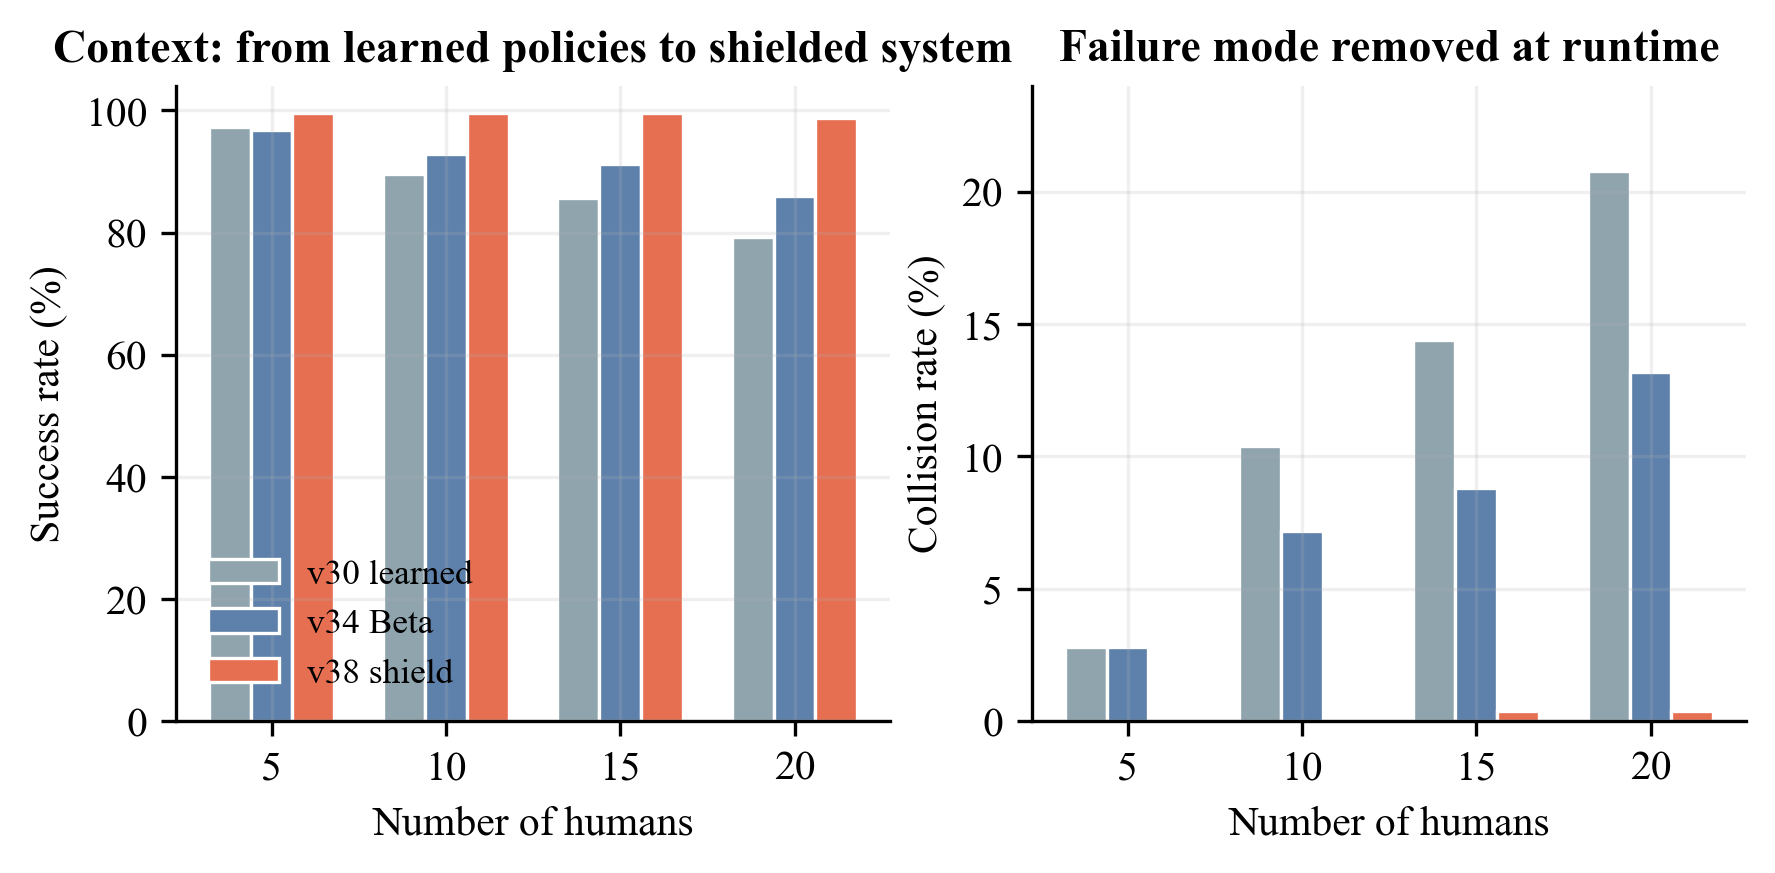
\includegraphics[width=\columnwidth]{fig_v38_context.png}
\caption{Bağlam karşılaştırması. V30 ve v34 saf öğrenilmiş politikalardır; V38, v34 üzerine eklenen
çarpışma-risk filtresidir. Runtime kalkan bu değerlendirmede yüksek yoğunlukta çarpışma kipini güçlü biçimde
azaltır.}
\label{fig:context}
\end{figure}

\subsection{Yörünge örnekleri}
Şekil~\ref{fig:traj}, N=10 ve N=20 için V38 kalkanlı yörüngeleri gösterir. Robot kalabalığın içinden düz bir
çizgiyle geçmek yerine, yoğunluk arttıkça daha uzun ve kavisli rotalar üretir. Bu niteliksel sonuç,
Tablo~\ref{tab:final}'deki ortalama başarılı adım sayısıyla uyumludur.

\begin{figure}[H]
\centering
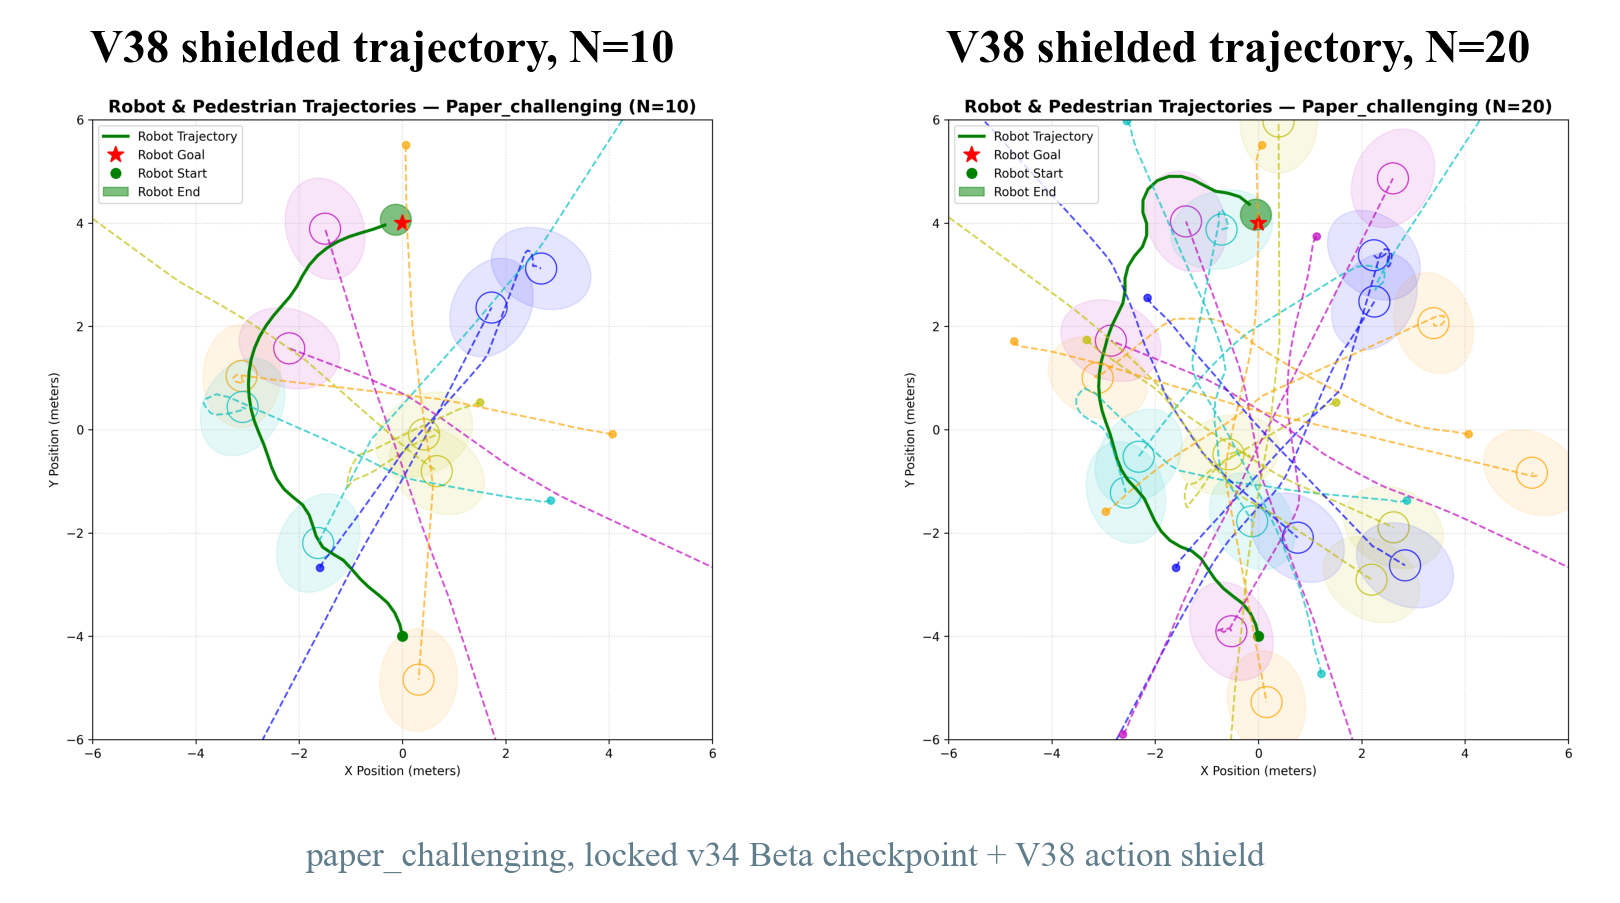
\includegraphics[width=\columnwidth]{fig_v38_trajectories.png}
\caption{V38 kalkanlı yörünge örnekleri. Kalkan, sosyal rotayı korur; yalnızca çarpışma sınırındaki eylemleri
değiştirir.}
\label{fig:traj}
\end{figure}

\begin{figure}[H]
\centering
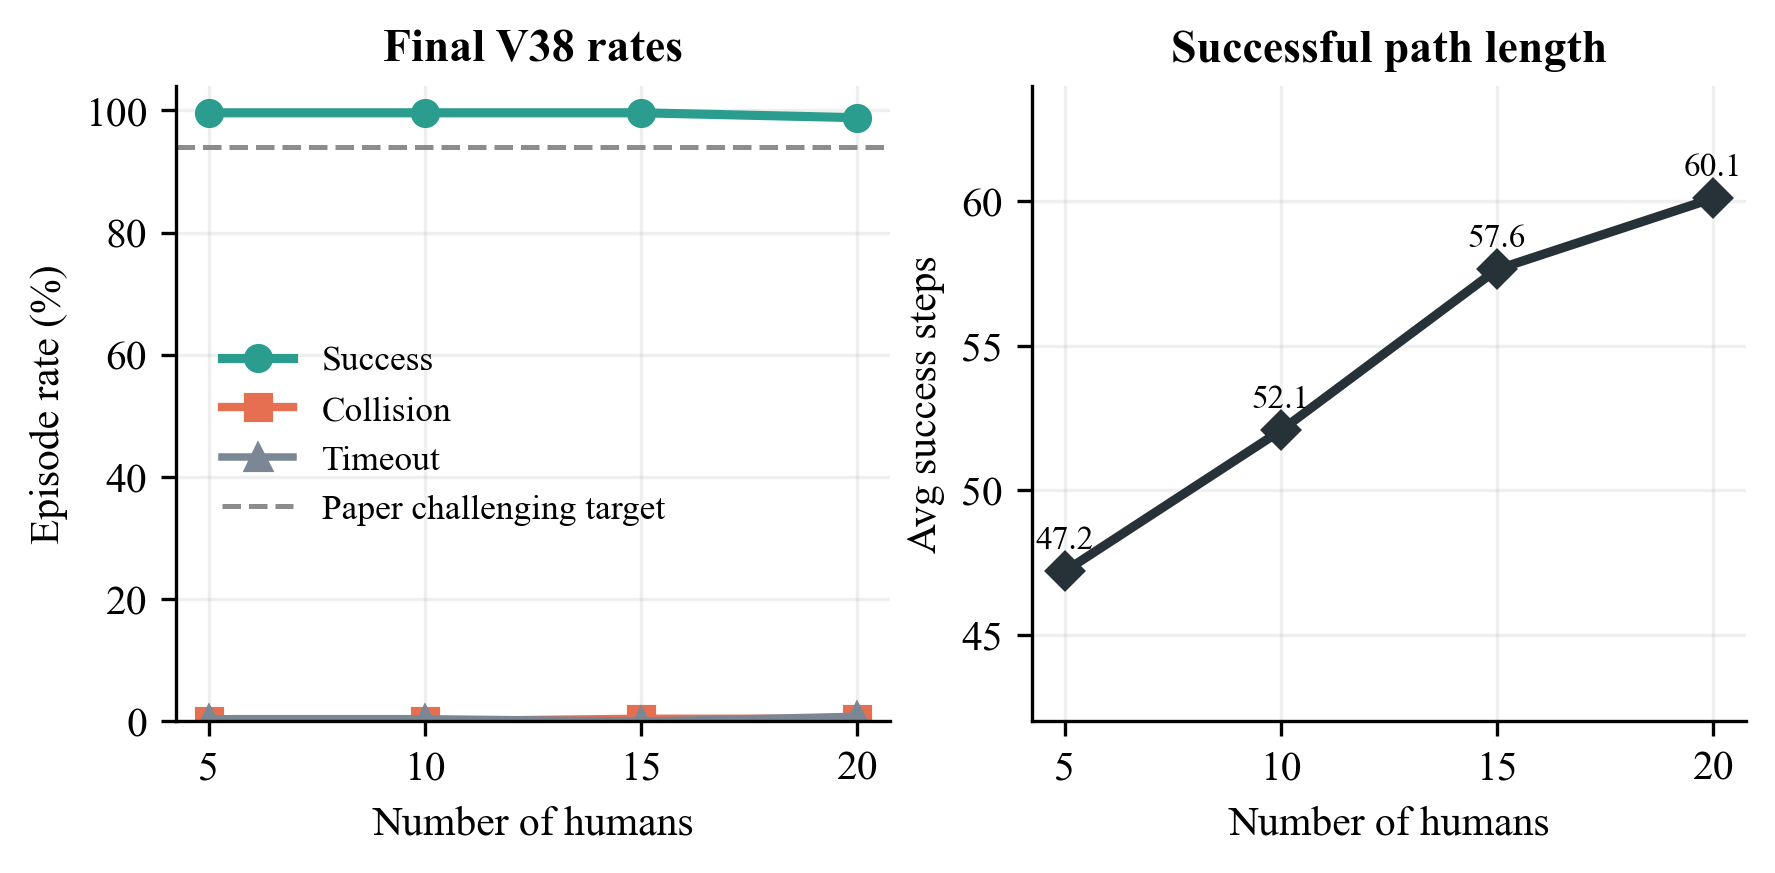
\includegraphics[width=\columnwidth]{fig_v38_final_sweep.png}
\caption{Final V38 yoğunluk sweep'i. Başarı yüksek kalır, çarpışma ve zaman aşımı düşük kalır. Başarılı yol
uzunluğu yoğunlukla arttığı için sosyal rota davranışı korunur.}
\label{fig:sweep}
\end{figure}

% =====================================================================
\section{Tartışma}
% =====================================================================
V38 sonucunun doğru okunması gerekir. Bu sistem yeni bir PPO checkpoint'i değildir. Öğrenilmiş bileşen v34
Beta politikasıdır; V38 bu politikanın yürütme zamanı eylemini çarpışma riski açısından denetler. Bu nedenle sonuç,
``daha iyi eğitilmiş saf SNCP'' değil, ``öğrenilmiş sosyal rota + analitik risk filtresi'' olarak
değerlendirilmelidir.

Bu ayrım pratik açıdan avantajdır. Yeni bir tam PPO eğitimi saatler sürebilir ve daha önce öğrenilmiş güçlü
davranışı bozabilir. V38 ise mevcut checkpoint'i korur ve yalnızca riskli eylem sınırında müdahale eder.
Eşleştirilmiş sonuçlarda düşük yoğunlukta anlamlı gerileme olmaması, yüksek yoğunlukta ise çarpışmanın
neredeyse sıfırlanması bu tasarım tercihini destekler.

V38'in sınırlamaları da açıktır. Kalkan kısa-horizon sabit-hız öngörüsüne dayanır; gerçek robotta bu öngörü
algılama gürültüsü ve gecikmeden etkilenebilir. ORCA yayaları bir sonraki adımda yön veya hız değiştirebildiği
için sabit-hız varsayımı bazen yanlış pozitif uyarı üretebilir ve gereksiz küçük rota düzeltmelerine neden
olabilir; daha nadir olarak ani yaya manevrası yanlış negatif risk de oluşturabilir. Kısa ufuk bu etkiyi
sınırlar, fakat gerçek zamanlı robot uygulamasında bu varsayım ayrıca test edilmelidir. Ayrıca V38 özellikle
challenging rejimdeki çarpışma kipini hedefler; standard senaryoda görülen zaman bütçesi kaynaklı hatalar ayrı
seçim veya ince ayar gerektirebilir. Sonuçlar tek kilitli v34 eğitim checkpoint'i üzerinde ve beş değerlendirme
tohumunda gösterilmiştir; farklı PPO eğitim tohumlarına genelleme ayrıca test edilmemiştir. Aynı bölüm bankası
üzerindeki eşleştirme için McNemar veya paired bootstrap gibi bölüm-düzeyi analizler gelecek çalışmada daha
uygun bir tamamlayıcı istatistik sağlayabilir. Gelecek iş olarak kalkan davranışı politikaya distile edilebilir
veya PPO eğitimi sırasında risk filtresi ile birlikte öğrenme denenebilir.

% =====================================================================
\section{Sonuç}
% =====================================================================
Bu makale, SNCP--PPO projesinin mevcut nihai durumunu V38 final sistemi olarak yeniden çerçeveler. Kilitli
v34 Beta politikası sosyal rota üreticisi olarak korunur; V38 action shield ise kısa-horizon çarpışma riskini
yürütme zamanında azaltır. Bu sonuç, öğrenilmiş sosyal rota üretimi ile analitik risk filtresinin birlikte
kullanılmasının, ek PPO eğitimi gerektirmeden pratik bir final sistem adayı verebildiğini gösterir.

\bibliographystyle{IEEEtran}
\bibliography{refs}

\end{document}
